\chapter{\IfLanguageName{dutch}{Stand van zaken}{State of the art}}
\label{ch:stand-van-zaken}
Smartphones bieden ons het voordeel dat we altijd en overal toegang hebben tot informatie. Toch kan niet iedereen die voordelen ten volle benutten.  Aanpassingen aan mobiele applicaties zijn noodzakelijk om zoveel mogelijk mensen die voordelen te geven. De mobiele platformen iOS en Android bieden een uitgebreid assortiment aan functionaliteiten om deze aanpassingen mogelijk te maken. Om een duidelijk beeld te krijgen over het probleemdomein, zal dit hoofdstuk beschrijven wat de huidige situatie rondom toegankelijkheid is. Wat de verschillende beperkingen en mobiele platformen zijn.

%Om duidelijkheid een duidelijker beeld te scheppen over de huidige situatie rondom toegankelijkheid op mobiele platformen, zal dit hoofdstuk dieper ingaan op 


\section{Toegankelijkheid}
\label{sec:toegankelijkheid}
Toegankelijkheid kan voor velen vaak een abstract begrip zijn. Het is het bruikbaar maken van zowel de gewone wereld als de digitale wereld voor iedereen \autocite{anySurferWat}. In dit onderzoek zal de focus gelegd worden op het toegankelijk maken van de digitale wereld. Meer bepaald het bruikbaar maken van mobiele applicaties. Want mobiele applicaties bieden ons net als websites toegang tot communicatie, informatie, educatie en nog veel meer \autocite{introAccesibilityw3c}. Toegankelijkheid in de digitale wereld wordt steeds belangrijker, de digitale revolutie zorgt ervoor dat steeds meer informatie digitaal wordt overgebracht. Mensen die nood hebben aan toegankelijkheid slagen er niet in om die informatie op de daarvoor voorziene manier te bekomen. Er zijn aanpassingen nodig voor die doelgroep ook toegang te bieden aan die informatie.
Wanneer men niet slaagt in het correct toepassen van aanpassingen voor het toegankelijker maken van digitale informatie, dreigt een deel van de doelgroep uitgesloten te worden.





\subsection{Wetgeving}
\label{sec:wetgeving}
Dankzij wettelijke bepalingen zal in sommige gevallen ontwikkelaars verplicht worden om hun applicaties toegankelijker te maken. Want toegankelijkheid zorgt ervoor dat mensen met een beperking ook kunnen functioneren in onze maatschappij. De wetgeving behoed men ervan om deze groep dan ook te vergeten. 

Door de geschiedenis heen zijn er verschillende verdragen en wettelijke bepalingen vastgelegd. De belangrijkste worden hieronder besproken. 




\subsubsection{Verdrag inzake rechten van personen met een handicap}
Het verdrag die op 13 december 2006 door de Verenigde Naties (VN) goedgekeurd is, heeft als doel dat mensen met een beperking evenveel rechten heeft als iemand anders, en daarbij ook ondersteund wordt om deze rechten te bekomen.  Het VN-Comité kijkt erop toe dat het verdrag gerespecteerd wordt. Niet voldoen aan deze richtlijnen kan gezien worden als het discrimineren van een individu \autocite{unia2006}. 

Binnen de omvang van dit onderzoek is vooral  \textbf{artikel 9} van belang. Dit artikel beschrijft hoe de ondertekende landen mensen met een beperkingen moeten faciliteren tot het toegankelijker maken van functioneren in de samenleving. Hieronder valt betere toegang tot informatie, toegang tot communicatie, toegang tot nieuwe technologieën, etc.. \autocite{un2006}

%Nog iets over belgie hier?
\subsubsection{The European Accessibility Act}
De Europese Commisie wil met de European Accessibility Act (EAA) de ongeveer 80 miljoen mensen met een beperking volledige en gelijke participatie in de gemeenschap garanderen. 

Binnen verschillende lidstaten van Europa werd het verdrag van de Verenigde Naties (VN) geïmplementeerd, met elk zijn eigen regelgeving omtrent toegankelijkheid.
Handel van producten en diensten met aanpassingen voor toegankelijkheid tussen verschillende lidstaten verloopt moeizaam, dit doordat elke lidstaat een specifieke regelgeving heeft.
Dit zorgt voor een barrière voor het implementeren van aanpassingen bij producten die verhandeld worden in meerdere lidstaten.

De EAA is bedoeld om in alle lidstaten binnen Europa dezelfde functionele vereisten te stellen aan producten en diensten. Met als doel toegankelijkheid makkelijker implementeerbaar te maken, dankzij die vaste set van vereisten. 
Als voordeel dat mensen met een beperking toegankelijkere producten hebben, en bedrijven in elke lidstaat dezelfde set van vereisten hebben.

Lidstaten worden verplicht de EAA te implementeren. Maar voldoen bij het succesvol implementeren ook aan het verdrag opgesteld door de VN \autocite{eaa2015}.



\subsubsection{Directive (EU) 2016/2102}
De richtlijn 2016/2102 van het Europese parlement van 26 oktober 2016 richt zich op het verhogen van de toegankelijkheid van digitale informatie afkomstig van overheidsinstanties. De richtlijn benadrukt het belang van toegankelijkheid doordat de digitale maatschappij zich steeds meer ontwikkelt, en de 'digitale agenda' van Europa die onlinecontent probeert te bevorderen speelt hier ook een grote rol in. De informatie die beschikbaar wordt gesteld door overheden moet dus op een niet-discriminerende manier beschikbaar worden gemaakt. 

Zowel websites als mobiele applicaties van overheidsinstanties moeten voldoen aan de toegankelijkheidseisen die gesteld worden. Verschillende lidstaten hebben zelf een invulling gegeven aan toegankelijkheidseisen. Toch wil deze richtlijn een aantal gemeenschappelijke eisen voor alle lidstaten opleggen. Dit zorgt ervoor dat ontwikkelaars en ontwerpers minder obstakels hebben, en kosten kunnen dalen op gebied van toegankelijkheid.

De richtlijn stelt ook dat indien mogelijk zou alle content/informatie toegankelijk moeten zijn, anders zou er een toegankelijk alternatief moeten zijn. Websites en mobiele applicaties van overheidsinstanties moeten toegankelijk gemaakt zijn door ze waarneembaar, bedienbaar, begrijpelijk en robuust te maken.
 
Er wordt verwacht van de lidstaten dat mobiele applicaties van overheidsinstanties voldoen aan deze richtlijn tegen 23 juni 2021 \autocite{directive2016}.

\subsection{W3C WAI toegankelijkheid standaarden/richtlijnen}
\label{sec:standaarden}
De W3C (World Wide Web Consortium) is een organisatie die standaarden probeert voor te schrijven voor het web. Een onderdeel van deze organisatie is het W3C Web Accessibility Initiative (WAI), zij hebben als doel het toegankelijker maken van het web
 \autocite{introAccesibilityw3c}. De standaarden beschreven door W3C omtrent toegankelijkheid worden gezien als internationale standaarden, en zijn ook het vertrekpunt voor de diverse Europese normen en richtlijnen.
 
De W3C WAI zijn vooral gericht op webapplicaties en web pagina's, toch kunnen de richtlijnen \textbf{WCAG 2.0} toegepast worden op alle soorten mobiele applicaties. Dit komt doordat vaak de user interface van mobiele applicaties vergelijkbaar is met web applicaties. Toch bieden mobiele applicaties een groot aantal toegankelijkheids-tekorten die anders zijn dan web applicaties \autocite{w3mobileConsider}. Gedurende dit onderzoek zullen wij ons grotendeels baseren op deze richtlijnen, omdat deze een internationale standaard zijn.

Het is belangrijk te weten dat er geen aparte richtlijnen voor mobiele applicaties zijn, deze zijn allemaal opgenomen in de WCAG richtlijnen. \textbf{WCAG 2.1} gepubliceerd in juni 2018 bevat wel extra criteria gericht op mobiele applicaties.
\autocite{w3cMobileGuidelines}

\subsection{Doelgroep}
\label{sec:doelgroep}

Een zeer groot aandeel van de mensen die nood hebben aan aanpassingen aan mobiele applicaties zijn mensen met een beperking.  Uit cijfers van \cite{who2018} blijkt dat ongeveer 15\% van de wereldpopulatie  een vorm van een beperking heeft. Dit is een grote groep, die zeer waarschijnlijk ook gebruik maken van mobiele applicaties. Deze groep zijn permanent beperkt.

De redenen waarom aanpassingen nodig zijn voor mensen met een beperking zijn heel divers, de verschillende beperkingen worden verder in dit hoofdstuk besproken.

Senioren behoren ook tot onze doelgroep, die krijgen vaak te maken met ouderdomsverschijnselen. Die zorgen ervoor dat ze ook beperkt kunnen zijn in hun dagelijks functioneren. Het onderzoek van \cite{diaz2014accessibility} bevestigt dat er aandacht moet besteed worden aan de oudere generatie, om uitsluiting te voorkomen. Aanpassingen voor senioren zou hun ook meer stimuleren om technologie te gebruiken.


Een ander belangrijk aandeel zijn mensen zonder beperkingen. Hieronder vallen mensen met een tijdelijke beperking, bijvoorbeeld een gebroken arm. Maar ook diegene met een situatie beperking, bijvoorbeeld dronken zijn \autocite{inclusiveMicrosoft}. Voor zowel tijdelijke als situatie beperkingen kunnen aanpassingen zeer hartelijk zijn.  Een voorbeeld hiervan is het gebruik van spraakbesturing wanneer men aan het autorijden is.

\begin{figure}[h]
    \centering
    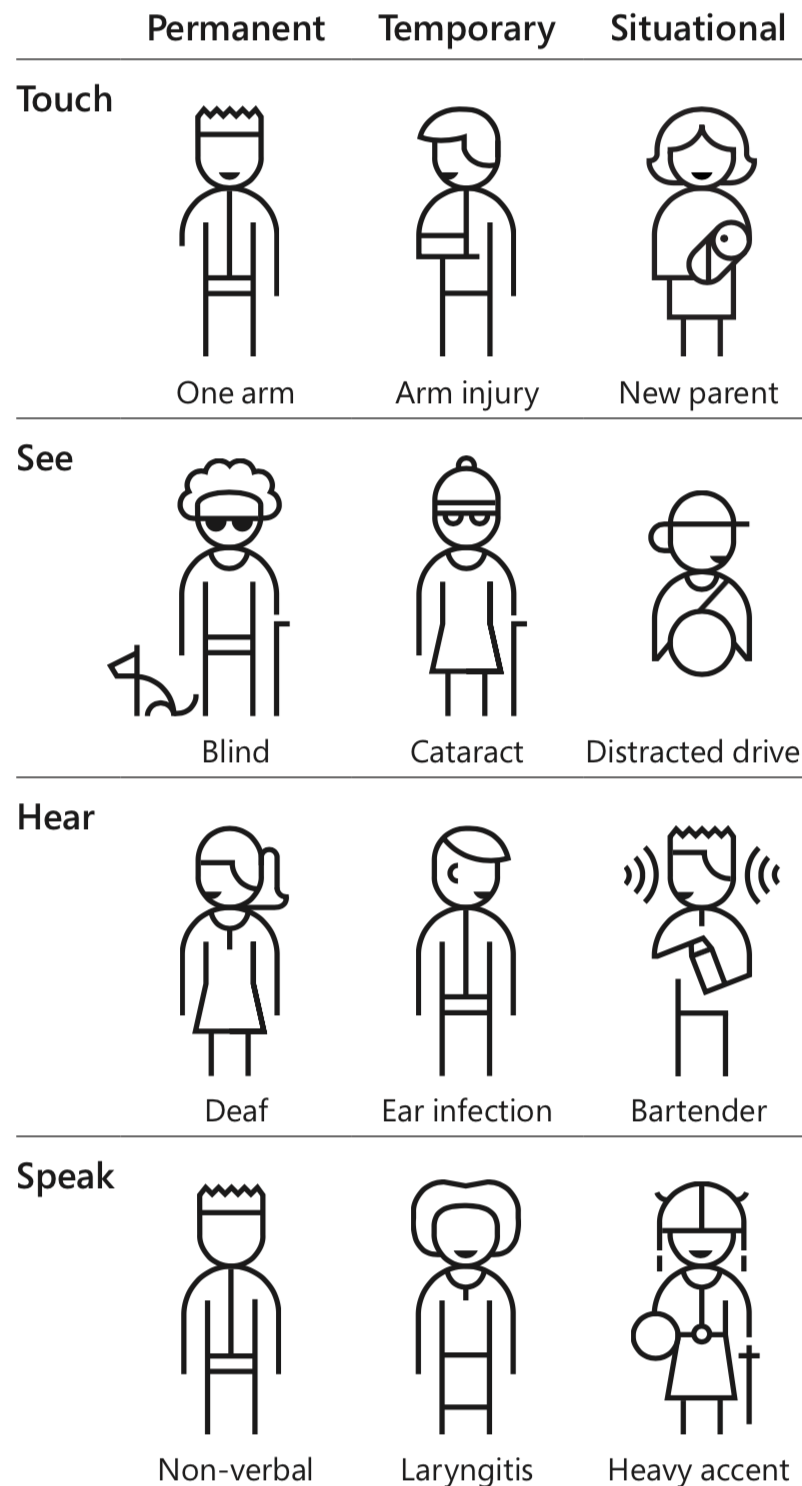
\includegraphics[width=0.4\linewidth]{img/doelgroep_situatie_tijdelijk}
    \caption{Persona spectrum \autocite{inclusiveMicrosoft}}
\end{figure}





\section{Beperkingen}
\label{sec:beperkingen}
Om inzicht te krijgen hoe toegankelijkheid verhoogd kan worden, is ook kennis over de verschillende beperkingen nodig. Er zijn veel verschillende beperkingen, in dit onderzoek worden ze per type gegroepeerd. Deze types zijn vernoemd naar de functie die beperkt wordt.
De verschillende types beperkingen behandeld in dit onderzoek zijn respectievelijk: 
\begin{itemize}
    \item Visueel
    \item Auditief
     \item Motorisch
     \item Cognitief
    \end{itemize}


De term beperking beschrijft het gelimiteerd zijn in uitvoeren van activiteiten of het hebben van bepaalde restricties. \autocite{whoDis2019}. Dit door het beperkt zijn in het uitvoeren van bepaalde lichaamsfuncties. En dit op een tijdelijke of permanente basis. Vaak is ook ondersteuning nodig voor het te kunnen functioneren zoals dat wenselijk is.

\subsection{Visueel}
\label{sec:Visueel}
Een zeer belangrijke lichaamsfunctie is het zicht, dankzij dit zintuig kunnen we verschillende prikkels waarnemen. Toch is niet iedereen in staat om op een normale manier deze prikkels waar te nemen. Het zicht kan beperkt zijn, waarbij dat ook nog sterk kan variëren in sterkte en oog. Dit op tijdelijke of permanente tijdsbasis \autocite{accessibility2019}.

\subsubsection{Kleurenblindheid}
Iemand die kleurenblind is, die ziet nog kleuren, maar niet op een correcte manier. De meeste mensen worden met kleurenblindheid geboren, maar kan ook veroorzaakt worden door ziekten.
Het type kleurenblindheid dat het meeste voorkomt is rood-groen stoornis, bij ongeveer 8,00\% van de mannen, en 0,04\% bij vrouwen. 

Ons lichtgevoelige cellen in ons netvlies zijn verantwoordelijk voor omzetting van kleur naar onze hersenen. En door het niet goed functioneren van enkele van die cellen ontstaat er kleurenblindheid. We noemen de cellen verantwoordelijk voor die omzetting van kleur ook wel kegeltjes. Een defect in de hersenen kan ook de oorzaak zijn voor kleurenblindheid. 

Figuur \ref{fig:ballenbak} toont 3 belangrijke soorten kleurenblindheid. Ze hebben de volgende kenmerken: 
\begin{itemize}
    \item \textbf{Protanoop}: rode kleur waarneming verstoord.
    \item \textbf{Deuteranoop}: groene kleur waarneming verstoord..
    \item \textbf{Tritanoop}: blauwe kleur waarneming verstoord.
\end{itemize}

Het verschil in de soorten kleurenblindheid ligt in het aantal en soort kegeltjes die niet correct functioneren \autocite{visioKleur2019}.



\begin{figure}[!h]
    \centering
    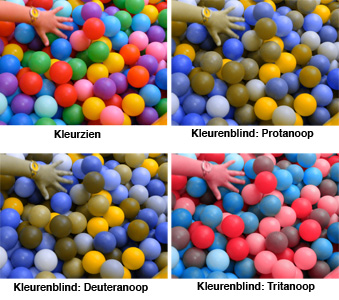
\includegraphics[width=0.5\linewidth]{img/ballenbak}
    \caption{Visuele voorstelling soorten kleurenblindheden \autocite{visioKleur2019}.}
    \label{fig:ballenbak}
\end{figure}



\subsubsection{Slechtziend en blindheid}
Men spreekt van slechtziendheid wanneer het gezichtsvermogen sterk is verminderd en niet oplosbaar is. Er gesproken van zwaar slechtziendheid wanneer men een gezichtsscherpte heeft van maximaal 30,00\% of een klein gezichtsveld heeft die kleiner of gelijk is aan 20 graden. Er bestaan heel veel soorten slechtziendheid. Zo kan iemand heel wazig zicht hebben door een zwakke gezichtsscherpte, of tunnelzicht door een klein gezichtsveld.

 Er wordt gesproken van blindheid wanneer men maximaal 5,00\% gezichtsscherpte meer bezit. Dit betekent dat men nog zicht heeft, maar heel beperkt. Ook wanneer men een gezichtsveld heeft van maximaal 10 graden spreekt men van blindheid \autocite{LiLi2019Blind}.




\subsubsection{Verhogen toegankelijkheid}
Bij mensen die lijden aan blindheid of slechtziendheid kan vaak gekeken voor het gebruiken van andere zintuigen, zoals het voelen en het horen. In smartphones zal men vooral gebruik maken van geluid om de toegankelijkheid te verhogen.
Kleurenblindheid kan worden ondersteund door het contrast van gebruikte kleuren te verhogen, of zelfs kleuren benoemen helpt bij het gebruik van een smartphone \autocite{visioKleur2019}.


\subsection{Auditief}
\label{sec:Auditief}

Een ander belangrijk zintuig is het gehoor. Het laat ons ook toe om prikkels van geluid op te nemen. Mensen met een auditieve beperking hebben moeite met het waarnemen van deze prikkels. Dit kan zich uiten in het slechthorend zijn, of doof zijn. Ongeveer 5\% van de wereldpopulatie lijdt aan een auditieve beperking \autocite{whoDAHL2019}.

\subsubsection{Slechthorend en doof}
 Wanneer men niet in staat is  waar te nemen wat een persoon met normaal gehoor kan waarnemen wordt gezien als slechthorend. Slechthorendheid kan voorkomen in één oor, of beide oren. Men spreekt van slechthorendheid wanneer men in een volwassen oor een verlies van meer dan 40 decibel heeft, in een kinderoor een verlies van meer dan 30 decibel vergeleken met een goed horend persoon. Het beperkt een persoon in het normaal communiceren met anderen doordat er moeite is met het waarnemen van het gesprek \autocite{whoDAHL2019}.
  Doofheid is de toestand waarbij men aan een groot gehoorverlies lijdt die vaak onherstelbaar is. In dit geval moet gezocht worden naar alternatieve manieren voor te communiceren \autocite{accessibility2019}.

\subsubsection{Verhogen toegankelijkheid}
Voor het vervangen van audio bij het gebruik van mobiele applicaties kan men gebruik maken van tekst. Het ondertitelen, of transcripten van audio verhoogt de toegankelijkheid voor blinden en slechtzienden \autocite{accessibility2019}.

\subsection{Motorisch}
\label{sec:Motorisch}
Een motorische beperking, ook wel fysieke beperking genoemd is een toestand wanneer iemand een beperkte fysieke capaciteit en/of minder mobiel is. Bewegingen gaan hierdoor moeizamer dan anders. Een motorische beperking kan aangeboren zijn, maar kan ook komen door ziektes of een ongeval \autocite{achieveAU2019}.

\subsubsection{Verhogen toegankelijkheid}
Er zijn verschillende soorten beperkingen, waarbij ofwel geen handfunctie meer is, of die heel er verstoord is door bijvoorbeeld ongewenste bewegingen. Wanneer men hier last van heeft, kan het bedienen van een smartphone een grote uitdaging zijn. 
Kleine klikgebieden vervangen door grotere oppervlakten, voldoende tijd geven voor het uitvoeren van taken en nog veel meer kan mensen met deze beperking ondersteunen bij smartphone gebruik \autocite{accessibility2019}.







\subsection{Cognitief}
\label{sec:cognitief}
Cognitieve beperkingen zijn beperkingen die zorgen voor mentale, leer en/of psychologische limietringen. Onder de term cognitief beperkt vallen vele verschillende soorten beperkingen. In dit onderzoek gaan we ons beperken tot:
\begin{itemize}
    \item Gedragsstoornissen
    \item Neurologische stoornissen 
\end{itemize}

Er bestaan een groot aantal gedragsstoornissen, maar bij het gebruik van een smartphone gaan personen met ADHD (Attention Defict Hyperactivity Disorder) of mensen met ADD (Attention Defict Disorder) vaak moeilijkheden hebben met het concentreren Autisme zorgt ervoor dat een individu moeite heeft met communiceren en interactie.

Bij neurologische stoornissen is er vaak een probleem in de hersenen. Epilepsie is een stoornis waarbij mensen zeer gevoelig zijn aan lichtflitsen. Andere voorbeelden van neurologische stoornissen is dementie, psychologische problemen, ... 
\autocite{patel2016mental}

\subsubsection{Verhogen toegankelijkheid}
Voor mensen met ADD of ADHD is het wenselijk om zoveel mogelijk afleidingen te voorkomen. Bij autisme moet men zorgen dat er een voorspelbare en eenvoudige inhoud is.  Consistentie is ook een zeer belangrijk voor mensen met autisme.

Wanneer men te maken heeft men neurologische stoornissen zoals epilepsie moet men vooral het gebruik van lichtflitsen beperken, of opties aanbieden om deze te beperken. Het gedrag van de applicatie zo voorspelbaar mogelijk maken en eventueel afbeeldingen gebruiken \autocite{accessibility2019}.



\section{Mobiele platformen}
\label{sec:mobielePlatformen}
De mobiele industrie kende in de afgelopen jaren een enorme groei. We zijn geëvolueerd naar een mobiele revolutie waarbij veel informatie altijd en overal beschikbaar is.

Het is niet de hardware van een smartphone, maar de software die het meeste invloed heeft op ons. Dankzij het mobiel platform op een smartphone kunnen we interactie hebben ermee. Het laat ons toe om te surfen op het web, applicaties te gebruiken en nog veel meer. Wanneer een mobiel platform toegankelijk genoeg is, kunnen mensen met een beperking zeker ook gebruik maken van deze voordelen.


Uit statistieken van \cite{statMobile2019} blijkt dat Android een marktaandeel heeft van 74,15\%, iOS volgt daarna met een marktaandeel van 23,28\%. Samen is dit goed voor een marktaandeel van 97,43\%. We kunnen dus aannemen dat we voldoende hebben met het voeren van dit onderzoek gericht op Android en iOS.

Uit de resultaten van een onderzoek van \cite{webAIMSurvey} valt af te leiden dat het gebruik van toegankelijkheidsvoorzieningen op mobiele apparaten zeer populair is. Op de vraag of er gebruik wordt gemaakt van een screen reader op een mobiel apparaat heeft van de 1770 respondenten 88,00 \%, positief geantwoord. 90,90\% van de respondenten die een beperking heeft gebruikt een screen reader.


Zowel Android en iOS hebben een grote set van functionaliteiten voor het verhogen van de toegankelijkheid. Hieronder zullen deze kort besproken worden. %TODO: vermelden hoofdstuk waar ze uitgebreid besproken worden
\subsection{Android}
Doorheen de jaren is het mobiele platform Android sterk gevolueerd, doorheen verschillende versies zijn nieuwe functionaliteiten uitgerold geadresseerd naar het verhogen van de toegankelijkheid. In de meeste gevallen wordt de accessibility Application programming interface (API) uitgebreid naar een nieuwe versie.
\label{sec:Android}



 
 \begin{table}[!h]
   % \usepackage{color}
       \centering
       \begin{tabular}{|l|l|} 
           \hline
           \textbf{Versienummer} & \textbf{Toevoegingen/aanpassingen}                                                                                                                                                                                                                                                                                                                                                                             \\ 
           \hline
           1.6                   & \begin{tabular}[c]{@{}l@{}}\begin{tabular}{@{\labelitemi\hspace{\dimexpr\labelsep+0.5\tabcolsep}}l}Introductie screenreader 'Pico'\\Introductie accessibility framework\end{tabular}\end{tabular}                                                                                                                                                                                                              \\ 
           \hline
           4.0                   & \begin{tabular}[c]{@{}l@{}}\begin{tabular}{@{\labelitemi\hspace{\dimexpr\labelsep+0.5\tabcolsep}}l}Talkback ondersteunt navigatie met vinger (explore-by-touch)\\Mogelijkheid tot vergroten tekst\\Activeren toegankelijkheid functionaliteiten met een touch gebaar\\Webbrowser bevat screenreader~\end{tabular}\end{tabular}                                                                                 \\ 
           \hline
           4.2                   & \begin{tabular}[c]{@{}l@{}}\begin{tabular}{@{\labelitemi\hspace{\dimexpr\labelsep+0.5\tabcolsep}}l}Braille apparaten worden ondersteunt\\Verbeterde detectie van touch gebaren\end{tabular}\end{tabular}                                                                                                                                                                                                       \\ 
           \hline
           4.3                   & \begin{tabular}{@{\labelitemi\hspace{\dimexpr\labelsep+0.5\tabcolsep}}l}User interface (UI) automation framework voor testen UI\end{tabular}                                                                                                                                                                                                                                                                   \\ 
           \hline
           4.4                   & \begin{tabular}[c]{@{}l@{}}\begin{tabular}{@{\labelitemi\hspace{\dimexpr\labelsep+0.5\tabcolsep}}l}Ondersteuning voor ondertitelingen\\Verbeterde beschrijving van elementen voor TTS\end{tabular}\end{tabular}                                                                                                                                                                                                \\ 
           \hline
           5.0                   & \begin{tabular}[c]{@{}l@{}}\begin{tabular}{@{\labelitemi\hspace{\dimexpr\labelsep+0.5\tabcolsep}}l}\textcolor[rgb]{0.125,0.129,0.141}{Kleuren inverteren of tekst contrast verhogen}\\\textcolor[rgb]{0.125,0.129,0.141}{Scherm aanpassen voor betere differentiatie kleuren}\end{tabular}\end{tabular}                                                                                                        \\ 
           \hline
           7.0                   & \begin{tabular}[c]{@{}l@{}}\begin{tabular}{@{\labelitemi\hspace{\dimexpr\labelsep+0.5\tabcolsep}}l}Settings toegankelijkheid in setup besturingssysteem\\Grote van iconen en foto's kunnen veranderd worden\\Mono uitvoer van geluid\\Instelbare snelheid van TTS\end{tabular}\end{tabular}                                                                                                                    \\ 
           \hline
           8.0                   & \begin{tabular}[c]{@{}l@{}}\begin{tabular}{@{\labelitemi\hspace{\dimexpr\labelsep+0.5\tabcolsep}}l}API uitbreiding voor het maken van custom features\\Hardware shortcut voor toegankelijkheid feature te activeren\\Gebaren op vingerprintsensor als invoermanier\\TTS in meerdere talen\end{tabular}\end{tabular}                                                                                            \\ 
           \hline
           9.0                   & \begin{tabular}[c]{@{}l@{}}\begin{tabular}{@{\labelitemi\hspace{\dimexpr\labelsep+0.5\tabcolsep}}l}Nieuwe attributen voor gebruik Talkback te vergemakkelijken\\Waarschuwen bij veranderingen van informatie\\API voor uitvoeren acties (screenshots, ...)\\Toegankelijkheidsmenu\\Mogelijkheid tot voorlezen tekst waargenomen door camera\\Audio die zich aanpast aan de omgeving\end{tabular}\end{tabular}  \\
           \hline
       \end{tabular}
      \caption{Updates Android toegankelijkheid functionaliteiten \autocite{AndroidReleases}.}
 \label{androidUpdates}
 \end{table}

De functionaliteiten die besproken werden in tabel \ref{androidUpdates} zijn belangrijk voor het verhogen van de toegankelijkheid van een applicatie. Voor sommige functionaliteiten te kunnen gebruiken in een applicatie moet de ontwikkelaar deze ondersteunen. Wat wel opvalt, is het feit dat Android een heel veel inzet op API's voor het implementeren van eigen toegankelijkheid functionaliteiten. 

\subsection{iOS}
\label{sec:iOS}
% Hier zeker P
% \usepackage{color}

Dit hoofdstuk bevat je literatuurstudie. De inhoud gaat verder op de inleiding, maar zal het onderwerp van de bachelorproef *diepgaand* uitspitten. De bedoeling is dat de lezer na lezing van dit hoofdstuk helemaal op de hoogte is van de huidige stand van zaken (state-of-the-art) in het onderzoeksdomein. Iemand die niet vertrouwd is met het onderwerp, weet nu voldoende om de rest van het verhaal te kunnen volgen, zonder dat die er nog andere informatie moet over opzoeken \autocite{Pollefliet2011}.
\begin{table}[h]
    \centering
    \begin{tabular}{|l|l|} 
        \hline
        \textbf{Versienummer} & \textbf{Toevoegingen/aanpassingen}                                                                                                                                                                                                                                                                                                                                                                                                                                   \\ 
        \hline
        3.0                   & \begin{tabular}[c]{@{}l@{}}\begin{tabular}{@{\labelitemi\hspace{\dimexpr\labelsep+0.5\tabcolsep}}l}\textcolor[rgb]{0.2,0.2,0.2}{Screen reader, VoiceOver}\\\textcolor[rgb]{0.2,0.2,0.2}{Zoom function}\\\textcolor[rgb]{0.2,0.2,0.2}{Black on white function to reverse~colours~for higher contrast}\\\textcolor[rgb]{0.2,0.2,0.2}{Mono audio uitvoer}\\\textcolor[rgb]{0.2,0.2,0.2}{\textcolor[rgb]{0.133,0.133,0.133}{Speak Auto-text}}\end{tabular}\end{tabular}  \\ 
        \hline
        5.0                   & \begin{tabular}[c]{@{}l@{}}\begin{tabular}{@{\labelitemi\hspace{\dimexpr\labelsep+0.5\tabcolsep}}l}Ledflitsen bij meldingen\\Aangepaste vibratiepatronen\\Functie om text te laten uitspreken\\Aangepaste elementteksten voor VoiceOver\end{tabular}\end{tabular}                                                                                                                                                                                                    \\ 
        \hline
        6.0                   & \begin{tabular}[c]{@{}l@{}}\begin{tabular}{@{\labelitemi\hspace{\dimexpr\labelsep+0.5\tabcolsep}}l}Beperkte toegang in applicaties\\Ondersteuning voor compatibele hoorapparaten\\Voiceover voor maps, AssistiveTouch, zoom\end{tabular}\end{tabular}                                                                                                                                                                                                                \\ 
        \hline
        7.0                   & \begin{tabular}[c]{@{}l@{}}\begin{tabular}{@{\labelitemi\hspace{\dimexpr\labelsep+0.5\tabcolsep}}l}Switch Control voor besturen toestel\\Aanpassen stijl ondertitelingen\\Handschrift invoer voor VoiceOver\end{tabular}\end{tabular}                                                                                                                                                                                                                                \\ 
        \hline
        8.0                   & \begin{tabular}[c]{@{}l@{}}\begin{tabular}{@{\labelitemi\hspace{\dimexpr\labelsep+0.5\tabcolsep}}l}Speak screen, voor het voorlezen van tekst\\Ondersteuning voor braille invoer\end{tabular}\end{tabular}                                                                                                                                                                                                                                                           \\ 
        \hline
        9.0                   & \begin{tabular}[c]{@{}l@{}}\begin{tabular}{@{\labelitemi\hspace{\dimexpr\labelsep+0.5\tabcolsep}}l}Touch accommodations voor het besturen met een motorische beperking\\Mogelijkheid voor herhalende taken te definiëren met Switch Control\\Mogelijkheid tot aanpassen~\textcolor[rgb]{0.196,0.2,0.2}{AssistiveTouch}\end{tabular}\end{tabular}                                                                                                                     \\ 
        \hline
        10.0                  & \begin{tabular}[c]{@{}l@{}}\begin{tabular}{@{\labelitemi\hspace{\dimexpr\labelsep+0.5\tabcolsep}}l}Vergrootglas met de camera\\Kleurenfilters voor kleurenblinden\end{tabular}\end{tabular}                                                                                                                                                                                                                                                                          \\ 
        \hline
        11.0                  &                                                                                                                                                                                                                                                                                                                                                                                                                                                                      \\ 
        \hline
        12.0                  &                                                                                                                                                                                                                                                                                                                                                                                                                                                                      \\
        \hline
    \end{tabular}
\end{table}




Je verwijst bij elke bewering die je doet, vakterm die je introduceert, enz. naar je bronnen. In \LaTeX{} kan dat met het commando \texttt{$\backslash${textcite\{\}}} of \texttt{$\backslash${autocite\{\}}}. Als argument van het commando geef je de ``sleutel'' van een ``record'' in een bibliografische databank in het Bib\LaTeX{}-formaat (een tekstbestand). Als je expliciet naar de auteur verwijst in de zin, gebruik je \texttt{$\backslash${}textcite\{\}}.
Soms wil je de auteur niet expliciet vernoemen, dan gebruik je \texttt{$\backslash${}autocite\{\}}. In de volgende paragraaf een voorbeeld van elk.

\textcite{Knuth1998} schreef een van de standaardwerken over sorteer- en zoekalgoritmen. Experten zijn het erover eens dat cloud computing een interessante opportuniteit vormen, zowel voor gebruikers als voor dienstverleners op vlak van informatietechnologie~\autocite{Creeger2009}.

\lipsum[7-20]
